\documentclass[a4paper, twoside]{article}
\usepackage[left=2cm, right=2cm, top=2cm, bottom=2cm, bindingoffset=1cm]{geometry}
\usepackage{graphicx}
\usepackage[czech]{babel}
\usepackage{parskip} %odstavce
\usepackage[utf8]{inputenc}
\usepackage{hyperref}
\usepackage{url}
\usepackage{subcaption}
\usepackage{siunitx}
\usepackage{float}

\usepackage{makeidx} %rejstřík - \index{pojem}
\makeindex

\usepackage{fancyhdr} %záhlaví, zápatí
\pagestyle{fancy}
\fancyhf{}
\fancyfoot[LE,RO]{\thepage}
\fancyhead[L]{Gymnázium Jihlava, Jana Masaryka 1}

\fancypagestyle{bezCislovani}{
  \fancyfoot{}
}

\begin{document}

\begin{titlepage}
    \thispagestyle{bezCislovani}
    \begin{flushleft}
        \vspace*{5cm}
        {\Huge \textbf{Fyzika v~Minecraftu} \par}
        {\Large seminární práce ze semináře z fyziky \par}
        \vspace{12cm}
        {\normalsize Barbora Vosáhlová, 6A6 \par}
        {\normalsize 2023/2024 \par}
    \end{flushleft}
\end{titlepage}

\newpage
\thispagestyle{empty}
\mbox{}
\newpage

\newpage
\setcounter{page}{1}
\thispagestyle{empty}
\section*{Anotace}
Tato seminární práce se zaměřuje na zkoumání a měření tíhové síly v~Minecraftu a výpočtu tíhového zrychlení způsobené touto silou a následného porovnání výsledku s~reálným světem.

\section*{Abstract}
This seminar work focuses on exploring and measuring the force of gravity in Minecraft, calculating the gravitational acceleration caused by this force, and subsequently comparing the results with the real world.

\newpage
\thispagestyle{empty}
\mbox{}
\newpage

\newpage
\thispagestyle{empty}
\vspace*{\fill} 
\section*{Prohlášení}
Prohlašuji, že jsem seminární práci zpracovala samostatně pod vedením Mgr.~Ladislava Karla a uvedla jsem všechny použité zdroje informací.
\vspace{2cm}

\begin{flushright}
\begin{tabular}{@{}p{5cm}@{}}
\hline
\\
\centering Podpis \\
\end{tabular}
\end{flushright}

V Jihlavě dne \underline{\hspace{4cm}}

\newpage
\thispagestyle{empty}
\mbox{}
\newpage

\newpage
\thispagestyle{empty}
\vspace*{\fill} 
\section*{Poděkování}
Děkuji vedoucímu seminární práce Mgr.~Ladislavu Karlovi za pomoc s~výpočty a metodické vedení práce.

\newpage
\thispagestyle{empty}
\mbox{}
\newpage

\newpage
\thispagestyle{empty}
\tableofcontents

\newpage
\thispagestyle{empty}
\mbox{}
\newpage

\newpage
\section{Úvod}
Minecraft, jedna z nejpopulárnějších videoher všech dob~\cite{indian-tv-statistics}, je sandboxová hra z roku 2009, odehrávající se v~otevřeném světě~\cite{minecraft-wikipedia}. Svět Minecraftu nabízí hráči velkou svobodu pohybu, činnosti a interakcí s~okolním světem, což vznáší otázku – řídí se tento kostičkový svět reálnými fyzikálními zákony? Proto jsem se rozhodla porovnat fyzikální jevy a zákony ve~virtuálním světě Minecraftu s~těmi ve skutečném světě. V~průběhu této práce chci zkoumat, jak Minecraft zachází s~koncepty jako je gravitace, akustika a další fyzikální jevy.

\section{Historie Minecraftu}
Minecraft vytvořil Markus Persson, též známý pod přezdívkou \index{Notch} Notch. První prototyp této hry vznikl již v~roce 2005 pod názvem Cave Game, ovšem k dnešní verzi Minecraftu to mělo ještě velmi daleko. Ve hře šlo jen pokládat a ničit bloky a pohybovat se po herním světě, což byla v~této verzi rovina tvořená travnatými bloky. 

Přestože prvotní verze neměla velký úspěch, Markus Persson pokračoval ve vývoji a v~roce 2009 založil se svými přáteli firmu \index{Mojang} Mojang a hru vydali pod názvem Minecraft („Mine“ – těžit,  „Craft“ – vyrábět). Hra získala velký úspěch a začala rychle stoupat v~žebříčcích. Jeden z důvodů velkého úspěchu Minecraftu byli herní youtubeři, jelikož Minecraft patřil mezi málo her, které nebyly chráněny autorskými právy a tedy mohl být vysílán. 

S rostoucí popularitou hry ovšem začaly přicházet i větší problémy. Proto v~roce 2014 rozhodla tato skupina přátel prodat studio Mojang firmě Microsoft. Minecraft se nadále vyvíjí a aktualizuje s~pravidelnými aktualizacemi, které přidávají nové funkce, bloky a předměty do hry~\cite{minecraft-historie}.

\section{Gravitace}
\index{Gravitace}Gravitace, jakožto jedna z fundamentálních sil ve vesmíru, je síla přitažlivosti mezi hmotnými tělesy v~závislosti na hmotnosti a vzdálenosti. Tato síla je popsána Newtonovým zákonem gravitace, který říká, že síla mezi dvěma tělesy, která lze aproximovat jako body nebo jsou to homogenní sférická tělesa, je přímo úměrná jejich hmotnostem a nepřímo úměrná druhé mocnině vzdálenosti mezi nimi. Tato síla působí směrem ke středu tělesa a je zodpovědná za pád předmětů na zem a lze jí vyjádřit vztahem~\cite{newtonuv-gravitacni-zakon}
$$F_g = G\frac{m_1\cdot m_2}{r^2},$$
kde $F_g$ je gravitační síla,  $G$ je gravitační konstanta, $m_1$ je hmotnost prvního tělesa, $m_2$ je hmotnost druhého tělesa a $r$ je vzdálenost obou těles.

V Minecraftu je \index{Gravitace}gravitace také implementována, ovšem nepůsobí směrem ke středu světa. Minecraft je placka a hráč se může prokopat pod svět do nicoty. Ovšem gravitace nezmění směr a hráč padá donekonečna směrem dolů, přestože již tímto směrem není žádné těleso, které by mohlo působit gravitační silou. Gravitace také nepůsobí na všechny objekty. Gravitace působí jen na některé bloky, jako je písek či štěrk, na živé objekty a na předměty hráče. Proto právě tyto objekty budou terčem následujícího měření.

Jelikož se zeměkoule točí kolem své osy, nepůsobí na tělesa ve vztažné soustavě s~povrchem Země pouze gravitační síla, ale i síla odstředivá. Výslednice těchto dvou sil je tíhová síla. Ve světě Minecraftu ovšem žádná odstředivá síla nepůsobí, protože se nejedná o vesmírný objekt, ale o nekonečně velkou placku, která v~prostoru setrvává v~klidu. Proto jsou tíhová a gravitační síla v~Minecraftu totožné. 

Tíhová síla udává tělesům \index{Tíhové zrychlení}tíhové zrychlení. Tedy zrychlení, které působí na tělesa při volném pádu,
$$F_G = m\cdot g.$$
\index{Normálové tíhové zrychlení}Normálové tíhové zrychlení na zemi se rovná $g_0= \SI{9,80665}{\meter\per\second\squared}$. Udává se normálové tíhové zrychlení, jelikož Země se točí kolem své osy a tedy tíhové zrychlení není na všech místech stejné (největší je na pólech a nejmenší je na rovníku). Normálové tíhové zrychlení je hodnota tíhové zrychlení na 45° zeměpisné šířky u hladiny moře. Ovšem rozdíl v~tíhovém zrychlení na jednotlivých místech na Zemi je tak nepatrné, že je ve většině případů zanedbatelné. 

\index{Tíhové zrychlení}Tíhové zrychlení by mělo existovat i v~Minecraftu, ovšem mělo by být všude stejné. \index{Tíhové zrychlení}Tíhové zrychlení můžeme spočítat v~závislosti na čase volného pádu a vzdálenosti počáteční polohy předmětu od povrchu Země, tedy podle druhé pohybové rovnice, která je vyjádřit vztahem
$$d=\frac{1}{2}\cdot gt^2,$$
kde $d$ je vzdálenost počáteční polohy pádu předmětu od povrchu Země, $g$ je tíhové zrychlení a $t$ je doba pádu.

Tato rovnice ale zanedbává odpor vzduchu, proto by na Zemi nefungovala přesně. I v~Minecraftu by teoreticky měl existovat odpor vzduchu, jelikož v~něm existují stvoření jako papoušci, která mohou létat. Navíc se v~Minecraftu šíří zvuk, takže by tam měl existovat vzduch. V~takovém případě bychom museli použít složitější vzoreček na spočítání tíhového zrychlení, který nezanedbává odpor vzduchu~\cite{gravity-equation},
$$d=vt + \frac{v^2}{g}e^\frac{-gt}{v}-\frac{v^2}{g},$$
kde $d$ je vzdálenost počáteční polohy pádu předmětu od povrchu Země, $v$ je terminální rychlost, $t$ je doba pádu a $g$ je tíhové zrychlení.

\subsection{Měření v~Minecraftu}
Pro změření \index{Tíhové zrychlení}tíhového zrychlení v~Minecraftu je potřeba zjistit, jak dlouho trvá pád z určité výšky. Jelikož Minecraft není vytvořen za účelem měření fyzikálních vlastností, nejsou v~Minecraftu stejné jednotky jako v~realitě, proto budeme počítat v~jednotkách, které nám Minecraft nabízí. Jelikož celý Minecraftový svět je tvořen z kostek, které jsou stejně velké (vyjma některých dekorativních objektů), tak vzdálenost budeme měřit právě v~těchto blocích. 

Měření času je trochu složitější, neboť čas v~Minecraftu sice utíká, ale není jak ho přesně změřit. Proto budeme měřit čas alternativním způsobem. K měření času využijeme \index{Redstone}redstone. Redstone je objekt v~Minecraftu, který by se dal připodobnit k elektrickým vodičům v~reálném světě a slouží k vytváření obvodů a mechanismů. Koncept tohoto měření času je založen na bloku, přes který mohou propadávat předměty z jedné truhly do druhé v~konstantních intervalech, pokud do něj nejde žádný proud skrze redstone. Takže můžeme měřit čas podle počtu předmětů - v~tomto případě mrkví, které za daný čas propadnou.

Je důležité brát v~úvahu, že nejmenší jednotka ve které můžememěřit je jedna mrkev, což způsobuje určitou míru chybovosti v~měřeních. Pád tělesa totiž netrvá přesně celý počet mrkví, naměřený čas tedy nebude přesně odpovídat reálnému času.

\subsubsection{Zanedbaní odporu vzduchu}
Nejdříve jsem se pokusila spočítat tíhové zrychlení v~případě, že by při pádu tělesa na něj nepůsobili žádné disipativní síly.
Vytvořila jsem z redstonu obvod, který měří, jak dlouho trvá, než hráč dopadne na zem, v~závislosti na tom, kolik za čas pádu propadne mrkví, z jedné truhly do druhé. Obvod kontroluje, jestli je blok A zatížen. Pokud blok zatížen je, vysílá signál, takže mrkve nepropadnou z truhly D do truhly B. Ve chvíli, kdy se blok uvolní, přestane vysílat signál a předměty začnou propadávat.
K celému obvodu je přidána páčka E, která při sepnutí vysílá signál neustále, takže předměty nepropadávají nehledě na zatížení bloku. Slouží tedy k vypnutí celého obvodu. Viz~Obrázek~\ref{fig:obvod_mereni_g}.

\begin{figure}[H]
    \centering
    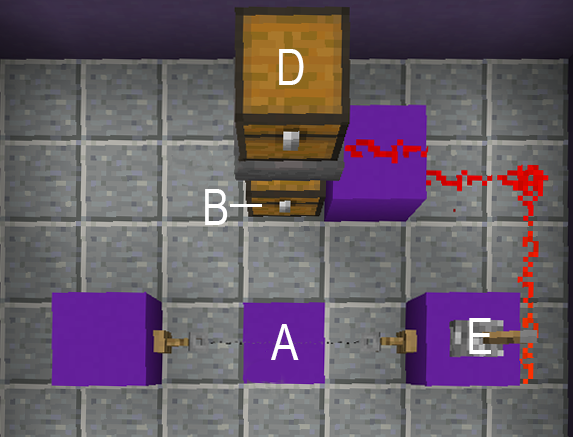
\includegraphics[width=0.5\textwidth]{g_obvod.png}
    \caption{Redstonový obvod pro měření tíhového zrychlení}
    \label{fig:obvod_mereni_g}
\end{figure}

Je však třeba, aby byl blok zatížen do chvíle, než hráč začne padat. Tedy aby se čas začal měřit přesně na začátku pádu. K tomuto účelu jsem využila příkaz k teleportaci na určité souřadnice. Postava hráče tedy stojí před teleportací na bloku A, hráče teleportujeme o určitý počet bloků vzhůru, tím přestane být blok zatížený a měření času začne přesně v~začátku pádu.

Následně jsem provedla měření času pádu hráče v~Minecraftu z různých výšek. Tato měření jsem prováděla z výšek od 50 bloků do 400 bloků v~intervalech po padesáti. Pro větší přesnost naměřených hodnot jsem měření pro každou výšku pádu opakovala osmkrát.

Aritmeticky průměrné doby pádu jsem poté dosadila do vzorečku pohybové rovnice $d = \frac{1}{2} gt^2$, kde $d$ představuje výšku pádu, $g$ značí hledané tíhové zrychlení a $t$ je čas pádu. 

\begin{figure}[h]
  \begin{subtable}{0.5\textwidth}
    \centering
    \begin{tabular}{c|c|c}
         d = [blok]& $t_p$ = [mrkev]  & g = [$blok\cdot mrkev^{-2}$] \\\hline
         50 & 4,75 & 4,43 \\
         100 & 7,38 & 3,68 \\
         150 & 9,25 & 3,51 \\
         200 & 11,40 & 3,09 \\
         250 & 13,40 & 2,80 \\
         300 & 15,50 & 2,50 \\
         350 & 16,90 & 2,46 \\
         400 & 18,50 & 2,34 \\
         
    \end{tabular}
    \caption{Tabulka naměřených hodnot}
    \label{tab:mereni}
  \end{subtable}
  \begin{subfigure}{0.4\textwidth}
    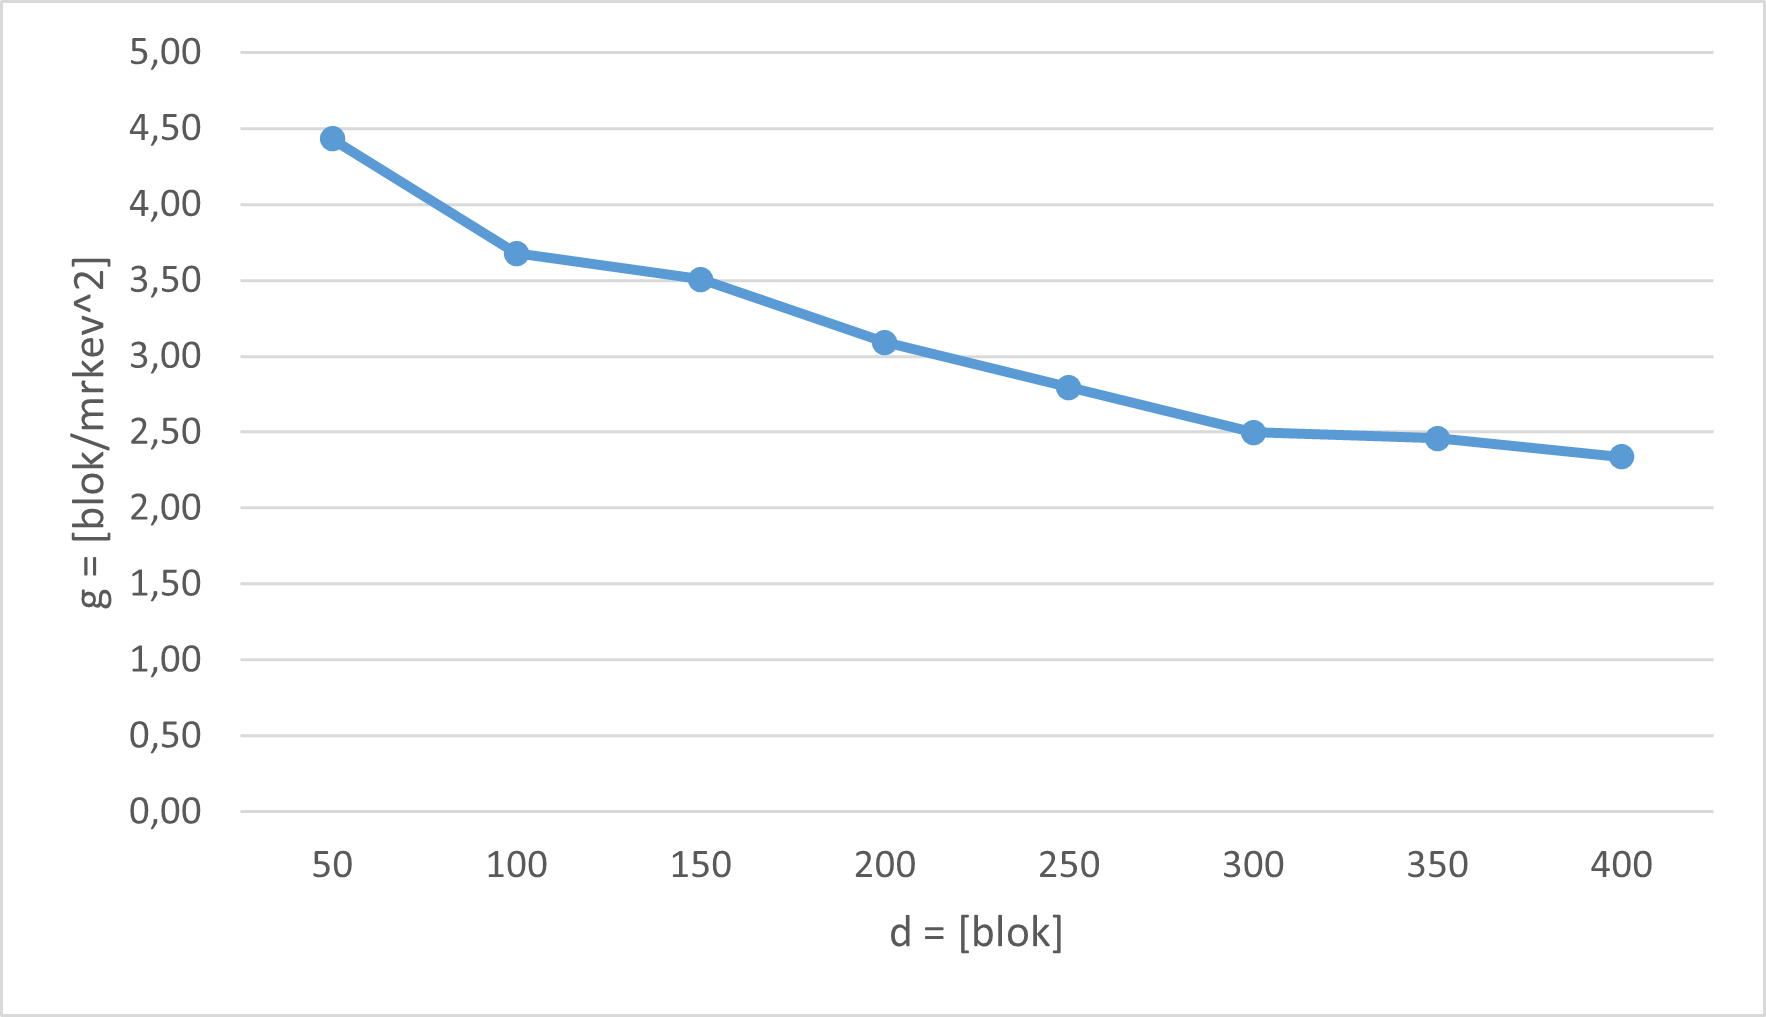
\includegraphics[width=\linewidth]{graf_g_zanedbani_odporu_vzduchu.png}
    \caption{Graf závislosti g(d)}
    \label{fig:graf_mereni}
  \end{subfigure}
  \caption{Měření tíhového zrychlení se zanedbáním odporu vzduchu}
  \label{fig:porovnani}
\end{figure}

Očekávané tíhové zrychlení by mělo být konstantní, nezávisle na výšce pádu, jelikož gravitační pole v~minecraftu je homogenní. Tedy gravitační síla a zrychlení, které tato síla způsobuje by mělo být všude stejné. Tento předpoklad ovšem nesouhlasí s~naměřenými daty, kde tíhové zrychlení klesá s~rostoucí vzdáleností počáteční polohy od země, viz~Obrázek~\ref{fig:porovnani}. Což znamená, že tento model tíhového zrychlení není správný a na padající objekt působí i jiné síly, než jen gravitační, které pád zpomalují.

\subsubsection{Uvažování odporu vzduchu}
Na padající tělesa tedy působí s~největší pravděpodobností i odpor vzduchu. Ten působí proti gravitační síle a tedy je výslednice sil menší, než gravitační síla a pád trvá déle. Odpor vzduchu je přímo úměrný rychlosti pohybu tělesa, tedy čím rychleji bude těleso padat, tím větší odpor vzduchu na něj bude působit. Zrychlení způsobené těmito silami můžeme spočítat přes vzorec $d=vt + \frac{{v_T}^2}{g}e^\frac{-gt}{v_T}-\frac{{v_T}^2}{g}$. Pro dosazení do tohoto vzorce je ovšem potřeba spočítat \index{Terminální rychlost}terminální rychlost, tedy maximální rychlost, které předmět dosáhne při volném pádu, protože tíhová síla se vyrovná odporové síle vzduchu. 

Pro výpočet terminální rychlosti bylo potřeba dosavadní obvod na měření doby pádu poupravit, aby měřil čas pádu posledních sto bloků, nezávisle na počáteční poloze hráče. Rychlost pádu na těchto posledních sto blocích se od určité výšky již nebude zvyšovat a zůstane konstantní, nehledě na počáteční polohu postavy. Vše ovšem komplikuje skutečnost, že  \index{Redstone} redston nemá nekonečný dosah. Přesně řečeno maximální dosah dráhy redstonu je 15 bloků a dál jeho signál nedosáhne. V~minecraftu sice existuje takzvaný \index{Repeater}repeater. Což je blok, která dokáže tento signál prodloužit na dalších 15 bloků, ovšem každý repeater způsobuje opoždění signálu. Což by značně komplikovalo měření času, jelikož bychom museli k naměřenému času přičítat opoždění způsobené těmito bloky a chybovost naměřených dat by byla ještě vyšší.

Proto do obvodu zapojíme \index{Command blok}command bloky, což jsou bloky, přes které lze vyvolávat ve hře příkazy pomocí příkazového řádku, který je v~těchto blocích zakomponován. Syntax těchto příkazů je specifický pro hru Minecraft. Většinou se využívají k automatizaci různých procesů, u kterých by byl redstone příliš prostorově náročný. V~minecraftu existují tři typy command bloků, které se dají rozlišit podle jejich barvy, viz~Obrázek~\ref{fig:typy_comm_bloku}.

\begin{figure}[H]
    \centering
    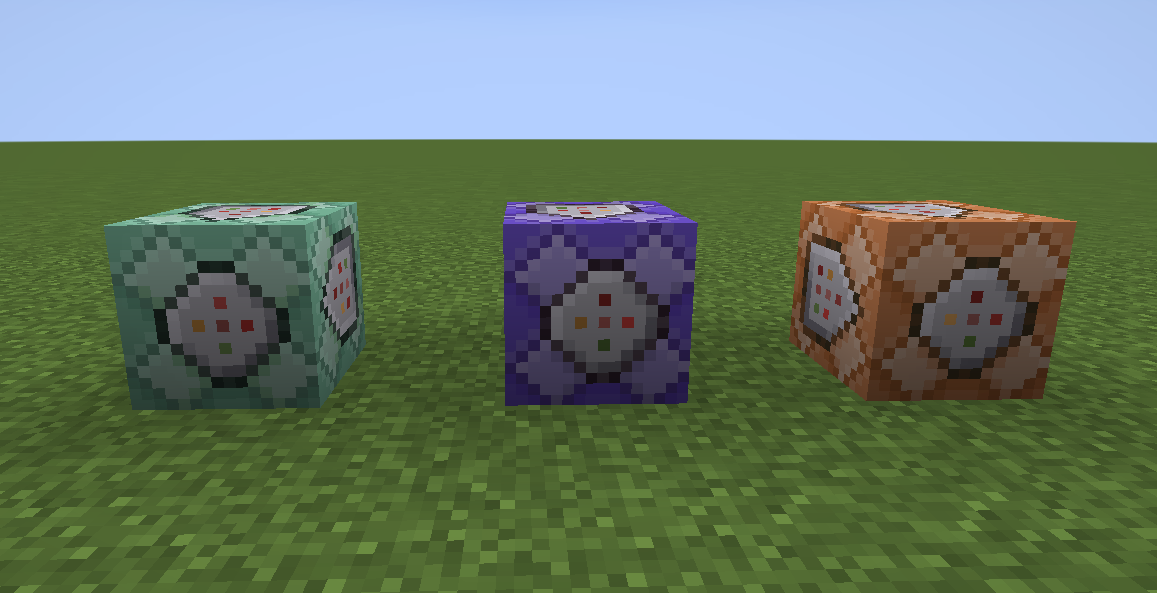
\includegraphics[width=0.6\textwidth]{Command_bloky.png}
    \caption{Typy command bloků}
    \label{fig:typy_comm_bloku}
\end{figure}

Základním typem je impulsní, který se značí béžovou barvou. Příkazy v~takovém command bloku se provedou jednou a pak se celý proces zastaví. Dalším typem jsou opakovací, fialové command bloky. V~takovém případě se budou příkazy neustále opakovat dokud není celý blok zastaven. Poslední variantou je řetězový, světle zelený. Tento typ pracuje s~principem, že jednotlivé command bloky se mohou řetězit za sebe (takové bloky musejí být umístěny vedle sebe, aby se dotýkaly stranami). Pořadí takto zřetězených command bloků určuje šipka, která je na nich nakreslená, viz~Obrázek~\ref{fig:navaznost}. Příkazy v~řetězovém bloku se spustí až po bloku na který navazují. Což umožňuje nastavovat složitější systémy.

\begin{figure}[h]
    \centering
    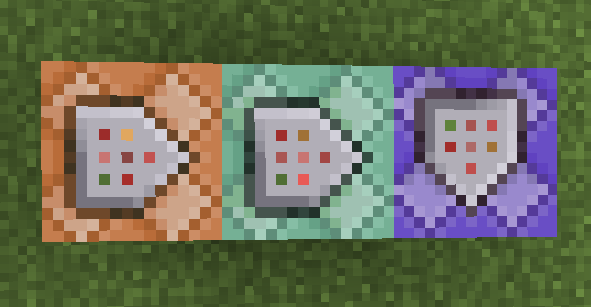
\includegraphics[width=0.5\textwidth]{posloupnost_comm_bloku.png}
    \caption{Řetězení command bloků}
    \label{fig:navaznost}
\end{figure}

Také se u těchto bloků dá nastavit podmíněnost. Toto nastavení ovšem ovlivní jen řetězové bloky. Podmíněnost určuje kdy proběhne příkaz. Pokud je blok podmíněný musí úspěšně proběhnout příkaz v~předchozím bloku nebo musí být například splněna podmínka v~předchozím bloku. Takové bloky nám tedy umožňují podmíněné programování v~rámci minecraftu. 
Dalším nastavením je potřeba redstonu, viz~Obrázek~\ref{fig:nastaveni}. Pokud je toto nastavení aktivní, tento blok nebude fungovat, pokud do něj nepůjde proud skrze redstone~\cite{command_blocks}.

\begin{figure}[h]
    \centering
    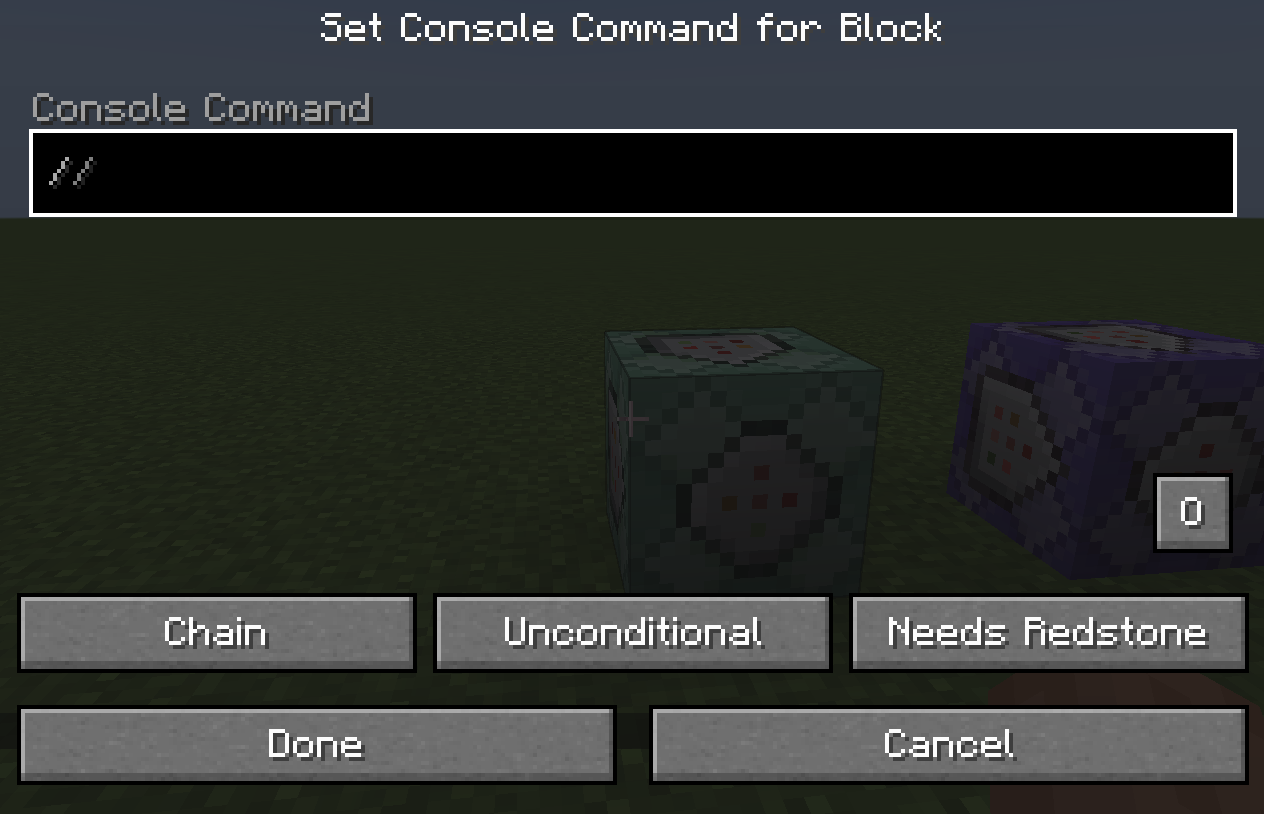
\includegraphics[width=0.6\textwidth]{command_block_settings.png}
    \caption{Nastavení command bloků}
    \label{fig:nastaveni}
\end{figure}

\newpage
Obvod, který měří dobu pádu za posledních 100 bloků, jsem vytvořila kombinací předchozí obvodu se dvěma command bloky. První tento blok přeruší obvod, pokud se hráč nachází sto bloků nad místem dopadu. Přerušením obvodu začnou propadávat mrkve, tedy se spustí časovač. Díky tomu se čas začne měřit až v~posledních sto blocích pádu. Původně měl tento command blok, spouštět senzor, který se spustí, když jím něco proletí (stejný senzor, který měří, že hráč dopadl na zem). Ovšem ukázalo se, že tento senzor dokáže zaregistrovat jen objekty do určité rychlosti. Terminální rychlost je vyšší, než je senzor schopný zaregistrovat a tedy se nespustil, když hráč proletěl. Z tohoto důvodu je command blok nastaven na opakování, tedy provádí příkaz neustále dokola a obvod se přeruší ve chvíli, kdy se hráč nachází právě těch sto bloků nad zemí.  
\begin{verbatim}
/execute if entity @a[x=17,y=39,z=1,dx=0,dy=0,dz=0] run setblock 19 -60 -2 air
\end{verbatim}

Při dopadu na zem se aktivuje senzor, který spustí příkaz v~druhém command bloku. Ten znovu obnoví celý obvod, takže mrkve přestanou propadávat.

\begin{verbatim}
/setblock 19 -60 -2 minecraft:redstone_block
\end{verbatim}

Následně jsem měřila rychlost pádu v~posledních sto blocích z různých výšek, počínaje počáteční výškou sto bloků. V~měřeních se ukazuje, že tato doba se po výšce 250 bloků již nemění a zůstává konstantní, viz~Obrázek~\ref{fig:terminální rychlost} Což znamená, že pád už nemůže být rychlejší, jelikož tíhová síla se vyrovná odporové síle vzduchu. Z naměřených dat tedy vyšlo, že terminální rychlost je $25~blok\cdot mrkev^{-1}$.

\begin{figure}[h]
    \centering
    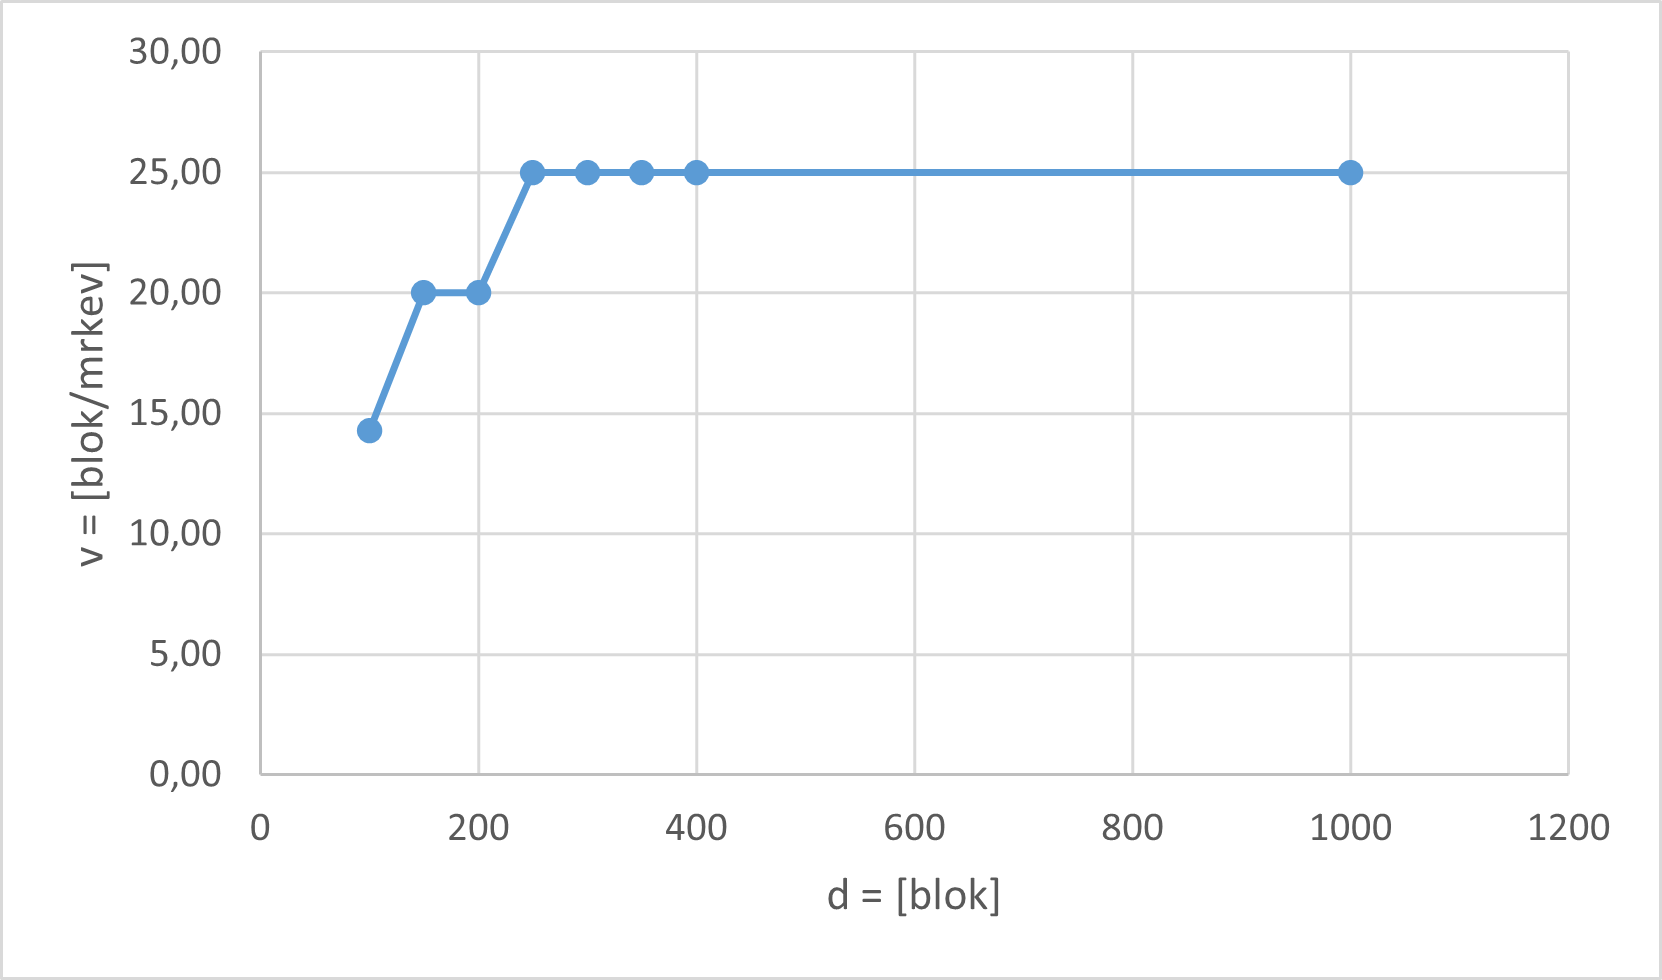
\includegraphics[width=0.6\textwidth]{terminalni_rychlost.png}
    \caption{graf závislosti v(d)}
    \label{fig:terminální rychlost}
\end{figure}

Po dosazení dat do vzorečku se ale ukázalo, že ani tento postup nedal žádný rozumný výsledek, jelikož tíhové zrychlení znovu nevyšlo konstantní, viz~Obrázek~\ref{fig:graf s odporem}. Výsledné zrychlení se u nízkých hodnot výšky pádu pohybuje okolo $7~blok\cdot mrkev^{-2}$, ale ve vyšších hodnotách výšky začne tíhové zrychlení vycházet nesmyslně.

\begin{figure}[h]
    \centering
    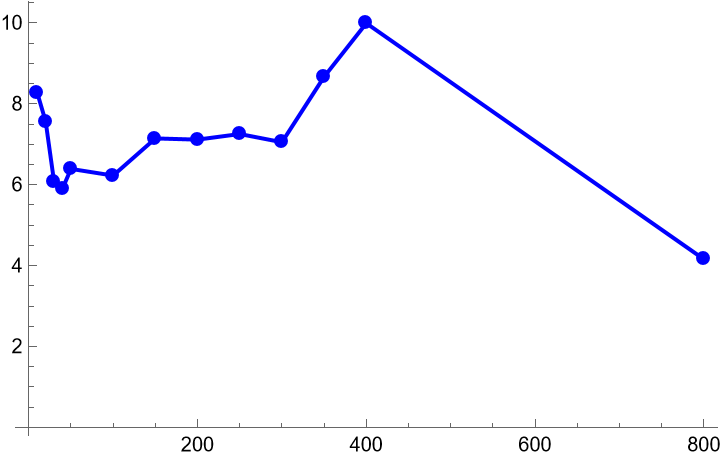
\includegraphics[width=0.6\textwidth]{tíhové_zrychlení_s_odporem.png}
    \caption{graf závislosti g(d) - s~odporem vzduchu}
    \label{fig:graf s odporem}
\end{figure}

\subsubsection{Statistická analýza}
Proto jsme se rozhodli data nafitovat, s~cílem na základě pozorovaných dat získat matematický model, který nejlépe popisuje tato data. 

První model, který jsme na fitování použili, byl model volného pádu, což je jednoduchý model pohybu v~tíhovém poli. Využili jsme vzorec pro výpočet výšky pádu v~závislosti na čase, stejně jako v~první části při zanedbání odporu.
$$y(t) \rightarrow \frac{g t^2}{2}$$

Druhým modelem je model s~odporovým členem, založený na Stokesově třecí síle. Tento model zohledňuje odpor vzduchu, který působí na padající objekt. Jeho rovnice jsou složitější a zahrnují parametr $k$, který reprezentuje odpor vzduchu. V~tomto modelu je třecí síla působící na těleso závislá na první mocnině rychlosti pádu.
$$y(t) \rightarrow \frac{g (-1 + e^{-k t} + k t)}{k^2}$$

Třetím modelem, který jsme zkoumali, byl model založený na Newtonově zákonu gravitace. Třecí síla je kvadraticky závislá na rychlosti. I tento model zahrnuje parametr $k$, kde $k = \frac{c s \rho}{2 m}$.
$$y(t) \rightarrow \frac{\ln (Cosh(t\sqrt{gk}))}{k}$$

Naměřená data jsme poté vložili do jednotlivých modelů, viz~Obrázek~\ref{fig:fitovani dat}. Tento postup nám umožnil porovnat výsledky a zjistit, který model nejlépe odpovídá našim pozorováním. Díky tomu jsme mohli lépe porozumět fyzikálním jevům a zákonitostem, které ovlivňují pád tělesa v~prostředí s~tíhovým polem.

\begin{figure}[h]
    \centering
    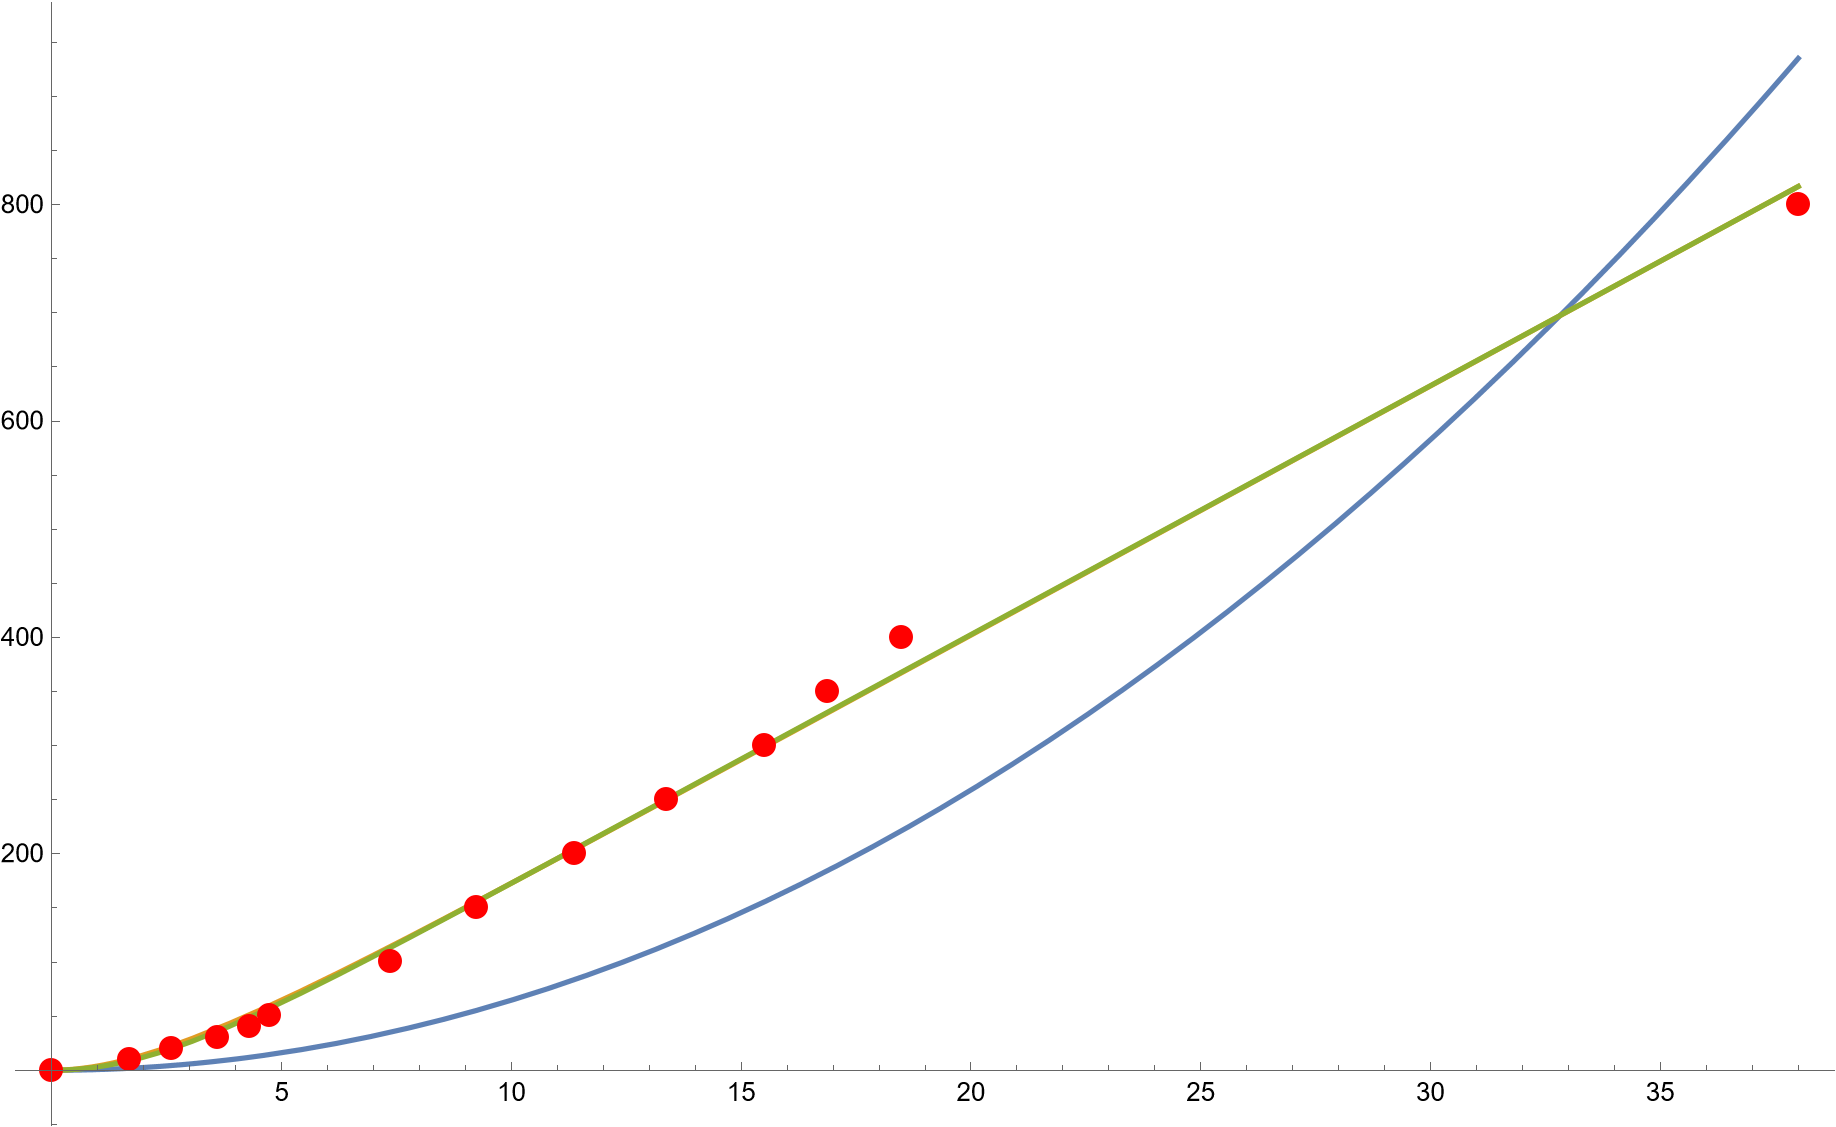
\includegraphics[width=0.6\textwidth]{fitovani_dat.png}
    \caption{Porovnání experimentálních dat s~teoretickými modely}
    \label{fig:fitovani dat}
\end{figure}

\begin{table}[h]
\centering
\begin{tabular}{|c|c|c|}
\hline
& Hodnota & Chyba \\
\hline
$g_0$ & $1.29531$ & $0.136689$ \\
\hline
$k_1$ & $0.393433$ & $0.060741$ \\
$g_1$ & $9.06386$ & $1.2236$ \\
\hline
$k_2$ & $0.0120684$ & $0.00186161$ \\
$g_2$ & $6.38843$ & $0.76071$ \\
\hline
\end{tabular}
\caption{Naměřené hodnoty a jejich chyby.}
\label{vypocitane hodnoty}
\end{table}

Z vypočtených hodnot vychází, že Minecraftu bude nejlépe odpovídat třetí Newtonův model, jelikož má nejnižší chybu a tedy nejvíce odpovídá naměřeným hodnotám, viz~Tabulka~\ref{vypocitane hodnoty}. Tyto výsledky také naznačují, že odpor vzduchu má významný vliv na pád v~Minecraftu. 

Výsledné tíhové zrychlení je tedy $g=6,38843~blok\cdot mrkev^{-2}$.

\subsection{Porovnání s~reálným světem}
Abychom mohli naměřenou hodnotu porovnat s~reálným světem, musíme hodnoty převést na stejné jednotky. Jelikož naměřené tíhové zrychlení je ve smyšlených jednotkách, které se nacházejí jen v~Minecraftu.

Minecraftový blok je čtverec s~obsahem jeden krychlový metr, tedy výška jednoho bloku je jeden metr~\cite{blok}. Pro převedení mrkví na sekundy jsem využila \index{Denní cyklus} denních cyklů. Protože celý jeden cyklus trvá dvacet minut~\cite{daylight-cycle}. Tento cyklus se dělí na denní a noční režim, kdy každý trvá přesně polovinu, tedy 10 minut. Celému obvodu, který měří dobu pádu jsem přidala senzor na denní světlo, který se zaktivuje jen v~noci, kdy nesvítí slunce. Tedy když začne den, obvod se přeruší a mrkve začnou propadávat. Propadávají celý denní cyklus, dokud se znovu nezaktivuje senzor. Díky tomu získáme přesný počet mrkví, které propadnou za 10 minut. Z experimentu vyšlo, že za 10 minut propadne 1510~mrkví, tedy jedna mrkev propadne za 0.397~sekund. Po převedení jednotek vyjde, že tíhové zrychlení v~Minecraftu je \SI{16.09}{\meter\per\second\squared}. Tedy tíhové zrychlení v~Minecraftu je větší než na Zemi. Můžeme tedy uvažovat, že svět Minecraftu působí na tělesa v~jeho gravitačním poli větší silou, než Země. Minecraftový svět byl měl tedy být těžší než Země.

\section{Závěr}
Provedená analýza naznačuje, že tíhové zrychlení v~Minecraftu se liší od hodnot, které bychom očekávali ve skutečném světě, ovšem odpovídá modelům a zákonům reality. Můžeme tedy říci, že i virtuální realita Minecraftu má své specifické fyzikální zákony. Tato práce úspěšně dosáhla stanoveného cíle a to spočítání tíhového zrychlení v~herním prostředí Minecraftu a jeho porovnání s~reálným světem.

Zároveň by se jistě dalo v~Minecraftu měřit a simulovat další fyzikální jevy, například zkoumat akustiku nebo hydrauliku, jelikož se tento svět řídí fyzikálními zákony a nabízí široké možnosti vytváření obvodů pro měření.






%---------------------------------------------------------------------

\newpage
\listoffigures 

\newpage
\renewcommand{\refname}{Použité zdroje}
\begin{thebibliography}{9}%\bibitem

\bibitem{indian-tv-statistics}%done
BURIAN, Michal.\textit{ Nejúspěšnější videohrou všech dob je Minecraft}. In: INDIAN, 22.~9.~2021 [online]. [cit. 2023-12-20]. Dostupné z: \url {https://indian-tv.cz/clanek/nejuspesnejsi-videohrou-vsech-dob-je-minecraft-se202d}

\bibitem{minecraft-wikipedia} %done
\textit{Minecraft}. In: Wikipedia: the free encyclopedia. San Francisco (CA): Wikimedia Foundation, 2001- [online]. [cit. 2024-01-16]. Dostupné z: \url{https://cs.wikipedia.org/wiki/Minecraft}.

\bibitem{minecraft-historie} %done
HORSKÝ, Dušan. \textit{Historie Minecraftu a studia Mojang}. In: Napojsa, 14.~3.~2020 [online]. [cit. 2023-09-24]. Dostupné z: \url{https://napojsa.sk/historie-minecraftu-a-studia-mojang}

\bibitem{newtonuv-gravitacni-zakon} %done
\textit{Newtonův gravitační zákon}. In: Wikipedia: the free encyclopedia. San Francisco (CA): Wikimedia Foundation, 2001- [online]. [cit. 2023-09-26]. Dostupné z: \url{https://cs.wikipedia.org/wiki/Newton%C5%AFv_gravita%C4%8Dn%C3%AD_z%C3%A1kon}

\bibitem{gravity-equation} %done
\textit{Equation of motion for free fall in a viscous fluid - Differential Equations} In:Youtube 19.~4.~2021 [online].  [cit. 2023-09-26]. Dostupné z: \url{https://www.youtube.com/watch?v=pJOyUPk8LfI&ab_channel=ThePhysicsMathsWizard}. Kanál uživatele The PhysicsMaths Wizard. 

\bibitem{command_blocks}
TRIUMPH BOOKS. \textit{The Ultimate Guide to Mastering Command Blocks!: Minecraft Keys to Unlocking Secret Commands}. 2016. Triumph Books. [Paperback]

\bibitem{blok} %done
\textit{Block}. In: Minecraft Wiki [online]. [cit. 2023-10-28]. Dostupné z: \url{https://minecraft.fandom.com/wiki/Block}


\bibitem{daylight-cycle} %done
\textit{Daylight cycle}. In: Minecraft Wiki [online]. [cit. 2023-10-28]. Dostupné z: \url{https://minecraft.fandom.com/wiki/Daylight_cycle}

\end{thebibliography} 

\renewcommand{\indexname}{Rejstřík pojmů}
\printindex

\end{document}

%poznámky:

